\section{Introduction}
\begin{figure}[th]
\centering
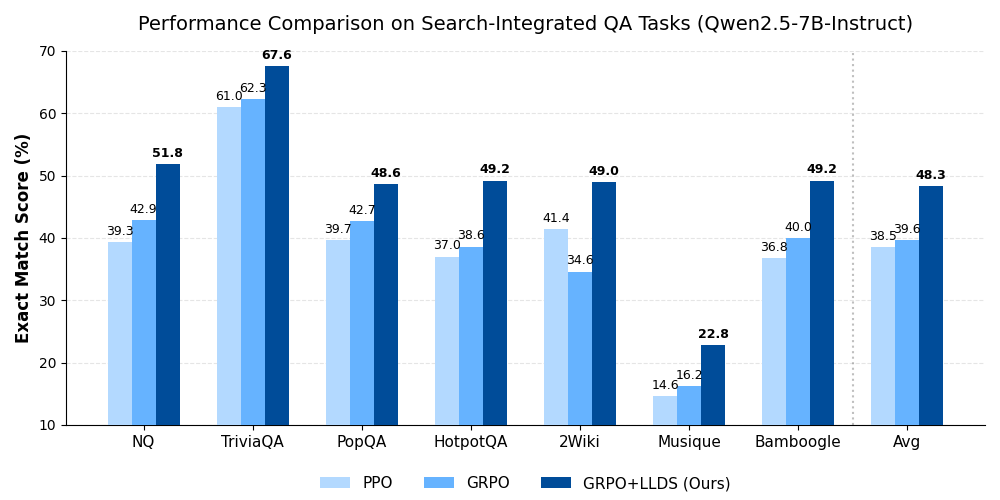
\includegraphics[width=\linewidth]{images/mainfig.png}
\caption{Comparative performance of LLDS and baseline methods on benchmark datasets. All baselines are built upon Qwen2.5-7B-Instruct. See~\cref{sec:reuslt} for details.}
\label{fig:7b_c}
\vspace{-3mm}
\end{figure}
Large language models (LLMs) increasingly leverage external tools, such as search engines~\citep{jin2025search} and code-execution environments~\citep{feng2025retool,zeng2025simplerl}, to augment their reasoning capabilities. This tool-integrated reasoning (TIR) paradigm has driven recent progress across factual question answering (QA)~\citep{jin2025search}, image-based reasoning~\citep{jiang2025verltool}, and mathematical problem solving~\citep{feng2025retool,jiang2025verltool}. By enabling models to iteratively query tools, tool calls substantially elevate reasoning quality~\citep{qin2023toolllm}. These advances naturally motivate the use of reinforcement learning (RL) to train LLMs to plan, interact with tools, and master multi-step decision making, as instantiated by TIRL frameworks such as Search-R1~\citep{jin2025search}.  
\\
However, extending TIR to the RL setting leads to severe and persistent training instabilities. In particular, GRPO training in Search-R1–style pipelines frequently suffers from abrupt reward drops and catastrophic collapse~\citep{jin2025search,sun2025zerosearch}. These failures are especially pronounced in multi-turn tool scenarios~\citep{xue2025simpletir}, where out-of-distribution tool feedback is incorporated into the model’s context. Although prior work observed these failures, the underlying mechanisms lack understanding.
\\
In this work, we first identify Lazy Likelihood Displacement (LLD)~\citep{deng2025effect,razin2024unintentional,ren2024learning}, the stagnation or reduction of likelihood for both correct and incorrect responses during GRPO optimization~\citep{deng2025effect}, as the fundamental but \textit{previously overlooked} source of collapse in TIRL. Using search-integrated QA as a case study (see~\cref{fig:dynamic}), we show that LLD emerges early and persistently: even as rewards increase, the likelihood of correct responses enters a monotonic decline. This behavior appears across model scales, indicating that LLD is a structural failure mode of GRPO-based TIRL rather than a configuration-specific artifact. We further demonstrate that LLD drives a self-reinforcing LLD death spiral, where the resulting low-confidence regime amplifies negative-gradient influence from incorrect trajectories, accelerating likelihood decay, triggering entropy spikes, inflating likelihood ratios, and ultimately causing the large-gradient instability that leads to collapse.
\\
To counteract this failure mode, we propose a simple yet effective LLD suppression (\ours{}) regularization that prevents harmful likelihood reductions. Our method integrates seamlessly with GRPO and introduces two layers of selectivity: (i)~\emph{action-level gating}, which activates the regularization only when a response action’s overall likelihood decreases, and (ii)~\emph{token-level selectivity}, which penalizes only the tokens responsible for the decrease. This fine-grained design directly mitigates LLD while minimally interfering with GRPO’s optimization behavior. By preventing unintentional downward likelihood drift, $\rm LLDS$ maintains stable training, suppressed gradient explosion, and consistent gains across seven open-domain and multi-hop QA benchmarks. Our main contributions are threefold:
\vspace{1mm}
\\
\noindent$\bullet$ We identify LLD as a previously unrecognized failure mode in GRPO-based tool-integrated reinforcement learning, and show that it arises pervasively and follows a consistent, self-reinforcing trajectory of sustained likelihood decay, gradient amplification, entropy explosion, and eventual training collapse.
% \xl{Suggested rephrase: We identify the \textbf{LLD Death Spiral}, a self-reinforcing collapse mechanism unique to tool-integrated GRPO, and characterize its three-phase progression: early stagnation, steady decay, and accelerated collapse. We show this phenomenon is driven by two structural factors absent in standard GRPO: (i) out-of-distribution tool feedback that systematically reduces action likelihood, and (ii) high prefix-similarity between correct and incorrect trajectories that amplifies conflicting gradients.}
\vspace{1mm}
\\
\noindent$\bullet$ We propose a lightweight regularization \ours{} that selectively regularize likelihood reductions and resolves the collapse issue in GRPO training.
\vspace{1mm}
\\
\noindent$\bullet$ By stabilizing training, we realize significant performance gains across QA benchmarks (see~\cref{fig:7b_c}), demonstrating a more robust and reliable approach to TIRL.
